%
% This is the LaTeX template file for lecture notes for EE 382C/EE 361C.
%
% To familiarize yourself with this template, the body contains
% some examples of its use.  Look them over.  Then you can
% run LaTeX on this file.  After you have LaTeXed this file then
% you can look over the result either by printing it out with
% dvips or using xdvi.
%
% This template is based on the template for Prof. Sinclair's CS 270.

\documentclass[twoside]{article}
\usepackage{amsmath}
\usepackage{amssymb}
\usepackage{float}
\usepackage{graphics}

\usepackage{xcolor,pifont}

\usepackage{tikz}
\usetikzlibrary{trees,positioning,arrows}

\setlength{\oddsidemargin}{0.25 in}
\setlength{\evensidemargin}{-0.25 in}
\setlength{\topmargin}{-0.6 in}
\setlength{\textwidth}{6.5 in}
\setlength{\textheight}{8.5 in}
\setlength{\headsep}{0.75 in}
\setlength{\parindent}{0 in}
\setlength{\parskip}{0.1 in}

%
% The following commands set up the lecnum (lecture number)
% counter and make various numbering schemes work relative
% to the lecture number.
%
\newcounter{lecnum}
\renewcommand{\thepage}{\thelecnum-\arabic{page}}
\renewcommand{\thesection}{\thelecnum.\arabic{section}}
\renewcommand{\theequation}{\thelecnum.\arabic{equation}}
\renewcommand{\thefigure}{\thelecnum.\arabic{figure}}
\renewcommand{\thetable}{\thelecnum.\arabic{table}}

%
% The following macro is used to generate the header.
%
\newcommand{\lecture}[4]{
   \pagestyle{myheadings}
   \thispagestyle{plain}
   \newpage
   \setcounter{lecnum}{#1}
   \setcounter{page}{1}
   \noindent
   \begin{center}
   \framebox{
      \vbox{\vspace{2mm}
    \hbox to 6.28in { {\bf EE 382V: Social Computing
                        \hfill Fall 2018} }
       \vspace{4mm}
       \hbox to 6.28in { {\Large \hfill Lecture #1, Session 1: #2  \hfill} }
       \vspace{2mm}
       \hbox to 6.28in { {\it Lecturer: #3 \hfill Scribe: #4} }
      \vspace{2mm}}
   }
   \end{center}
   \markboth{Lecture #1: #2}{Lecture #1: #2}
   %{\bf Disclaimer}: {\it These notes have not been subjected to the
   %usual scrutiny reserved for formal publications.  They may be distributed
   %outside this class only with the permission of the Instructor.}
   \vspace*{4mm}
}

%
% Convention for citations is authors' initials followed by the year.
% For example, to cite a paper by Leighton and Maggs you would type
% \cite{LM89}, and to cite a paper by Strassen you would type \cite{S69}.
% (To avoid bibliography problems, for now we redefine the \cite command.)
% Also commands that create a suitable format for the reference list.
\renewcommand{\cite}[1]{[#1]}
\def\beginrefs{\begin{list}%
        {[\arabic{equation}]}{\usecounter{equation}
         \setlength{\leftmargin}{2.0truecm}\setlength{\labelsep}{0.4truecm}%
         \setlength{\labelwidth}{1.6truecm}}}
\def\endrefs{\end{list}}
\def\bibentry#1{\item[\hbox{[#1]}]}

%Use this command for a figure; it puts a figure in wherever you want it.
%usage: \fig{NUMBER}{SPACE-IN-INCHES}{CAPTION}
\newcommand{\fig}[3]{
			\vspace{#2}
			\begin{center}
			Figure \thelecnum.#1:~#3
			\end{center}
	}
% Use these for theorems, lemmas, proofs, etc.
\newtheorem{theorem}{Theorem}[lecnum]
\newtheorem{lemma}[theorem]{Lemma}
\newtheorem{proposition}[theorem]{Proposition}
\newtheorem{claim}[theorem]{Claim}
\newtheorem{corollary}[theorem]{Corollary}
\newtheorem{definition}[theorem]{Definition}
\newenvironment{proof}{{\bf Proof:}}{\hfill\rule{2mm}{2mm}}

% **** IF YOU WANT TO DEFINE ADDITIONAL MACROS FOR YOURSELF, PUT THEM HERE:

\begin{document}
%FILL IN THE RIGHT INFO.
%\lecture{**LECTURE-NUMBER**}{**DATE**}{**LECTURER**}{**SCRIBE**}
\lecture{7}{November 9}{Vijay Garg}{Joshua Musick}
%\footnotetext{These notes are partially based on those of Nigel Mansell.}

% **** YOUR NOTES GO HERE:

% Some general latex examples and examples making use of the
% macros follow.  
%**** IN GENERAL, BE BRIEF. LONG SCRIBE NOTES, NO MATTER HOW WELL WRITTEN,
%**** ARE NEVER READ BY ANYBODY.
\section{Voting}
Voting is the aggregation of beliefs / rankings. Examples include gathering Concensus, or Search Engines.

If we consider a group of people on an island, and they all vote given two choices, it's easy to determine what is preferred by the majority.  But, when you add a third choice, it makes things complicated.  In particular if Alice gives the following preference for choices A, B, and C.

\begin{equation*}
 \text{\textcolor{red}{We have a Problem!}}
    \begin{cases}
        A > B \\
        B > C \\
        C > A
    \end{cases}
\end{equation*}

\begin{definition}[Plurality]
When chosing order, we want the following properties to produce a ranking.
\begin{enumerate}
    \item Transitivity - $\forall x, y, z : (x > y) \wedge (y > z) \implies (x > z)$
    \item Completeness - $\forall x, y : (x > y) \vee (y > x)$
\end{enumerate}
\end{definition}

\subsection{Sample Voting Ballot with Three Choices}
Each voter is represented by $V_i$, and the columns represent their preferences with their first choice on top, second below their first etc.

\begin{table}[H]
    \centering
     \begin{tabular}{ccc|c}
     $V_1$ & $V_2$ & $V_3$ & Final Ranking \\ \hline
     A & A & A & A \\
     B & B & C & B \\
     C & C & B & C 
    \end{tabular}
    \caption{Simple Case}
    \label{tab:ex1}
\end{table}
 
\begin{table}[H]
    \centering
     \begin{tabular}{ccc|c}
     $V_1$ & $V_2$ & $V_3$ &  \\ \hline
     A & B & C & (A $>$ B) : 2 \\
     B & C & A & (B $>$ C) : 2 \\
     C & A & B & (C $>$ A) : 2 
    \end{tabular}
    \caption{Problematic Case}
    \label{tab:ex2}
\end{table}

This lead to the discovery of \textbf{Condorcet's Paradox (1700's)}.

\begin{table}[H]
    \centering
     \begin{tabular}{c|c|c|c}
     College & National Rank & Class size & Money Offered  \\ \hline
     X & 4 & 40 & 3K \\
     Y & 8 & 18 & 1K \\
     Z & 12 & 24 & 8K 
    \end{tabular}
    \caption{Best College Example}
    \label{tab:ex3}
\end{table}

Voting in context of plurality is related to comparing 2 choices.  In Table~\ref{tab:ex3}, how do you decide which college is the best?

\section{Voting Systems}

\subsection{Axioms}

\begin{enumerate}
    \item \textbf{Unanimity} (U) \\
    If all voters prefer A over B, then in the final ranking, A must be placed over B.
    \item \textbf{Independence of Irrelevant Alternative} (IIA) \\
    For each pair of alternatives $x,y$ the group ranking should depend only on how each individual voter ranks $x$ and $y$ reltative to each other.
    \item \textbf{Non-Dictatorial} (ND) \\
    Voting system is not a Dictatorial system.
\end{enumerate}

\begin{table}[H]
    \centering
     \begin{tabular}{c|c|c}
     Critic & Unanimous Vote & IIA Vote \\ \hline
     $C_1$ & CK $>$ GF & CK $>$ GF $>$ PF \\
     $C_2$ & CK $>$ GF & CK $>$ GF $>$ PF \\
     $C_3$ & CK $>$ GF & CK $>$ GF $>$ PF \\
     $C_4$ & GF $>$ CK & GF $>$ PF $>$ CK \\
     $C_5$ & GF $>$ CK & GF $>$ PF $>$ CK 
    \end{tabular}
    \caption{Movie Preferences for Unanimous and IAA Votes}
    \label{tab:ex7}
\end{table}


In the first vote, (unanimous vote), CK is the obvious winner, 3 to 2.  In the second case, it is not so obvious.  If first choice gets 2 points, second 1 point, and third 0 points, the totals are as follows:

\begin{table}[H]
    \centering
     \begin{tabular}{c|c}
        Movie & Vote Totals \\ \hline
        CK & 6 \\
        GF & 7 \\
        PF & 2
    \end{tabular}
    \caption{Vote totals for IAA Example}
    \label{tab:ex8}
\end{table}


Once we add a third option, now the GF becomes the winner.  Furthermore, PF is also now an Irrelevant Alternative.

\subsection{Systems}

\newcommand{\xmark}{\textcolor{red}{\ding{55}}}%
\newcommand{\cmark}{\textcolor{green}{\ding{51}}}%

\begin{enumerate}
    \item \textbf{Majority Rule} [U \cmark] [IIA \xmark ] [ ND \cmark ]
    \\ A system where the option with the most votes or highest ranking is adopted.  This system can lead to the Condorcet Paradox
    \item \textbf{Positional Voting} [U \cmark] [IIA \xmark ] [ ND \cmark ]
    \\ This system uses Bordat Counting, to assign a number to each choice and the choice with the largest sum wins.  This does not solve the Condorcet Paradox, if selections are symmetric.
    
    \begin{table}[H]
    \centering
     \begin{tabular}{ccc|c}
     $V_1$ & $V_2$ & $V_3$ & Option Totals \\ \hline
     A (2) & A (2) & C (2) & A : 5 (winner) \\
     B (1) & C (1) & A (1) & B : 1 \\
     C (0) & B (0) & B (0) & C : 3 
    \end{tabular}
    \caption{Sample Positional Voting with Assigned Values for each choice}
    \label{tab:ex4}
\end{table}
    
    
\begin{table}[H]
    \centering
     \begin{tabular}{ccc}
     $V_1$ & $V_2$ & $V_3$  \\ \hline
     A  & B & C \\
     B  & C  & A \\
     C  & A  & B   
    \end{tabular}
    \caption{Symmetric Vote Choices}
    \label{tab:ex9}
\end{table}

As you reconsider Table~\ref{tab:ex9}, if we instead of summing point values (Bordat Counting), only compare two choices at a time, we create a new problem.  A problem of order matters, see below:

\begin{center}
\begin{tikzpicture}
\begin{scope}[xshift=-7.5cm,yshift=-5cm,very thick,
		node distance=1.6cm,on grid,>=stealth',
		block/.style={rectangle,draw,fill=cyan!20},
		comp/.style={circle,draw,fill=orange!40}]
   \node [comp]  (re)					{C};
   \node [comp]	 (cb)	[above=of re,xshift=-0.8cm] {A}  edge [->] (re);
   \node [comp]	 (ca1)	[above=of cb,xshift=-0.8cm]	{A} edge [->] (cb);
   \node [comp]	 (ca2)	[right=of ca1]			{B} edge [->] (cb);
   \node [comp]  (ca3)  [right=of cb] {C} edge [->] (re);
   

    \node [comp] (Aab) [right=of re,xshift=2.4cm]	{A};
    \node [comp] (Bb)  [above=of Aab,xshift=-0.8cm] {B} edge [->] (Aab);
    \node [comp] (Ba)  [right=of ca2,xshift=0.8cm] {B} edge [->] (Bb);
    \node [comp] (Ca)  [right=of Ba] {C} edge [->] (Bb);
    \node [comp] (Aa1) [right=of Bb] {A} edge [->] (Aab);
    
   \end{scope}
   \end{tikzpicture}
\end{center}

In the depiction above, which is comparing two elements at a time, and then comparing the winner to the next element, demonstrates the problem.  Outcomes will vary simply based on what order you perform your comparison.

\begin{definition}[Social Choice]
The top most choice.
\end{definition}
\begin{definition}[Social Welfare]
The complete ranking of all choices.
\end{definition}

Note: Each definition above can be deduced from the other...
    
    \item \textbf{Dictatorial}  [U \cmark] [IIA \cmark ] [ ND \xmark ]
    \\All voters agree with the dictator.
    
\end{enumerate}

\section{Arrow's Theorem}

\begin{theorem}[Arrow's Theorem]
There is no voting system that satisfies Unanimity, Independence of Irrelevant Alternatives, and Non-Dictatorial. - Kenneth Arrow (1950s)
\end{theorem}

\begin{definition}[Quorum]
$S$ is a quorum if all the members unanimously prefer $A$ over $B$ and all members not in $S$ prefer $B$ over $A$, then the final ranking places $A$ over $B$.
\end{definition}

\begin{lemma}
If $S$ is a quorum and $T$ is a quorum, then $S\cap T$ is a a quorum.

Given options $A, B,$ and $C$

$S$:  All voters prefer A to B and All voters in $S'$ prefer B to A.

$T$: All voters prefer B to C and all voters in $T'$ prefer C to B.

\centering
$A > B$ 

$B > C$

By transitivity, $A > C$ in final ranking.

Now focus on $S \cap T$:

$(S \cap T)^c = S^c \cap T^c$

$v = {w, x, y, z}$

$s_w={x,y,z}$

$s_x = {w,y,z}$

$s_y = {w,x,z}$

$s_z = {w,x,y}$

The intersection of all of these sets is the null set.

$\therefore$ All the axioms can not be met by any voting system.

\end{lemma}

\end{document}





